
\section{Two-Dimensional Liquid Crystal in Box Confinement}
\begin{itemize}
	\item Information on Onsager can be found on pg 59 of de Gennes/Prost
	\item Include other studies of the box confined LC	
	\item \textbf{Note} Page 31 of \cite{chen2016theory} mentions that the difference in the theoretic NI transition and experimental/simulated value is attributed to the higher virial terms contribute to free energy, which are absent in the Onsager model.
	\item See \cite{chen2016theory} page 24 for Onsager/hard rod stuff
	
\end{itemize}

In the following we look at the theoretic framework  and computational execution for finding stable configurations of the two-dimensional liquid crystal under a square confinement based off the work of X.~Yao, H.~Zhang, and J.~Z.~Y. Chen in Ref.~\cite{yao}. The configurations are produced as energy minima of an extended Onsager model. 

%We follow its derivation as layed out by de Gennes and Prost \cite{degennesbook} (pg.\ 59-62).
%For rod-like molecules of length $L$ and diameter $D$, the model makes the following assumptions:
%\begin{itemize}
%	\item The only relevant force is the steric repulsion of molecules, that is, a non-overlap interaction. Onsager also showed molecule Coulomb forces amount to increased effective molecule size.
%	\item The rods are long $(L\gg D)$
%	\item The volume fraction of rods $\Phi = cLD^2\pi/4\ll 1$ for rod concentration $c$.
%\end{itemize}

Since its publishing in 1949, the model put forth by Lars Onsager  \cite{onsager1949} has been a mainstay in describing the interaction of anisotropic colloidal particles, hence its popularity in studying the liquid cyrstal systems of rod or disk shaped molecules.
Here we focus our attention on the model as it applies to confined rod molecules under no external potential. Via this model we can gain insight into system properties, in particular \textbf{the I-N transition (maybe) and} solving for stable configurations.
Indeed this model was the launching point by which the rods-in-a-box configurations were solved for numerically in works \cite{yao,chen2013rods}.
The following is a quick explanation of the methods

To begin, we define a density distribution $\rho(\bv{r},\bv{u})$ where $\bv{r}$ represents the location of a given rod's center, and $\bv{u}$ its orientation. This density distribution is normalized such that $\int\rho(\bv{r},\bv{u})d\bv{r}d\bv{u} = N$.
The Onsager model then prescribes a free energy functional
\begin{align}
	\beta F = \int \rho(\bv{r},\bv{u}) \ln \left[ L^2\rho(\bv{r},\bv{u}) \right] d\bv{r}d\bv{u}
	+ \frac{1}{2} \int\rho(\bv{r},\bv{u}) w(\bv{r},\bv{u};\bv{r'},\bv{u'}) \rho(\bv{r'},\bv{u'}) d\bv{r}d\bv{u}d\bv{r'}d\bv{u'},
	\label{eq:onsagerfree}
\end{align}
where $\beta=1/k_BT$ for Boltzmann constant $k_B$ and temperature $T$. The first term relates to the positional and orientational entropies. Spatial entropy prefers a uniform distribution of particles, and orientational entropy prefers a uniform distribution of angles.
The second term emerges from the second-virial approximation and contains the interaction effects between molecules, represented by the kernel function $w(\bv{r},\bv{u};\bv{r'}\bv{u'})$. Via a Mayer cluster expansion, 
\begin{align}
	w(\bv{r},\bv{u};\bv{r'}\bv{u'}) = 1 - \exp\{-\beta \nu(\bv{r},\bv{u}; \bv{r'},\bv{u'})\},
\end{align}
where $\nu(\bv{r},\bv{u}; \bv{r'}\bv{u'})$ is our non-overlapping interaction potential
\begin{align}
	\nu(\bv{r},\bv{u}; \bv{r'},\bv{u'}) = 
	\begin{cases}
	+\infty & \text{if rods overlap}\\
	0 & \text{otherwise}
	\end{cases}
\end{align}

This means $w(\bv{r},\bv{u}; \bv{r'},\bv{u'}) = 1$ if rods overlap, increasing $F$, and $0$ if not. The interaction integral in \ref{eq:onsagerfree} can be simplified for a spatially homogeneous domain (with thin rods $D\ll L$) to
\begin{align}
	\int w(\bv{r},\bv{u}; \bv{r'},\bv{u'})dr'
	= L^2|\bv{u}\times\bv{u'}|,
\end{align}
(in two dimensions) as visualized in Fig [FIGURE]. Now it is clear that parallel rods optimize this orientation term. However, at the same time the entropy term is pushing for a uniform spread of angles and positions. From the competition of these terms then emerges the isotropic-nematic transition.

As discussed in \cite{chen2016theory} (pg.\ 25), truncating \ref{eq:onsagerfree} at the second virial term is quite valid in three dimensions---this was already resolved in Onsager's original work where he argued there was no need for higher-order terms for small $D/L$ systems---but is less appropriate in two dimensions where the higher-order terms are closer to the second order magnitude. This does render this equation for the free energy \textit{quantitatively} less accurate, but importantly the principal physics are still captured in this form. Indeed, this does underestimate the critical density of the I-N transition at $NL^2/A = 3\pi/2 \approx 4.71$, whereas the accepted value by experiment and simulation places it in the range $6-9$ [SOURCES].

In their work, Refs.\ \cite{chen2013rods,yao} determine numerical solutions from an mathematically equivalent self-consistent field theory model.  This model introduces a mean-field acting on rod segments and enacts Euler's forward scheme on a propagator of a modified diffusion equation to carry out the computation and locate energy minima. Additionally, special care was taken in incorporating the hard-wall boundary effects. This derivation is more involved and not essential for our purposes.

The two free phenomenological system parameters are the reduced density $\rho^* = NL^2/a^2$ and $L/a$ for box edge length $a$ \cite{chen2016theory}(in Ref.\ \cite{yao} a third is required, $b/a$, for rectangular width $b$).
The ratio $L/a$ is really a finite size scaling parameter, and the reduced density essentially determines the system topology of either isotropic or nematic, and the selection of (meta)stable states therein. 
Phase diagrams as functions of these three parameters are shown in Figure\ \ref{fig:phasediagram}. We can see that regardless of $b/a$ and $L/a$, a low enough reduced density will produce an isotropic state, and above which the specific nematic topology depends on all three parameters.

\begin{figure}
	\centering
	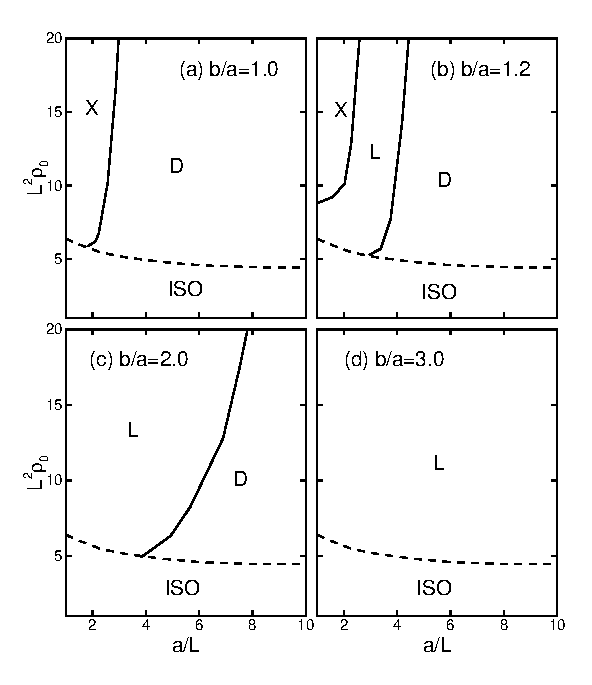
\includegraphics[width=0.7\textwidth]{./figs/ABCD.eps}
	\caption{Phase diagrams of the rectangular confined rod system from work \cite{yao} [PERMISSION?]. Here, $\rho_0 = N/a^2$ and the dashed line indicates a second-order phase transition.}
	\label{fig:phasediagram}
\end{figure}

\subsection{Orientational order}
Naturally, of great interest is a quantitative way to mark the whether a system is nematic of isotropic. That is, to mark when the higher symmetry of the isotropic phase is broken in the nematic phase. Qualitatively we describe this less symmetric nematic phase as having more order. The task then is to create an order parameter that vanishes to zero in the isotropic phase and approaches unity in the nematic phase.
For example, in a ferromagnetic system the magnetization is conveniently readily an appropriate order parameter. However, conjuring one for liquid crystals is less trivial.

We proceed with our derivation in three dimensions and then consider the two dimensional case. Naively one may opt for a directional average but since rods have a center of symmetry the average of $\bv{u}$ will cancel out. The next invariant is then the tensor
\begin{align}
	Q_{\alpha\beta} 
	= \frac{1}{N}\sum_i\left(u_\alpha^{(i)}u_\beta^{(i)} - \frac{1}{d}\delta_{\alpha\beta} \right),
\end{align}
in $d$ dimensions, where $\alpha$ and $\beta$ represent the Cartesian variables $x,y$ and $z$, $\delta_{\alpha\beta}$ is the Kroenecker delta, and the summation is a thermal average over a small but macroscopic volume. This $Q$-tensor has several useful properties:
\begin{itemize}
	\item It is symmetric since $u_\alpha^{(i)}u_\beta^{(i)} = 
	u_\beta^{(i)}u_\alpha^{(i)}$.\\
	
	\item It has zero trace:
	\begin{align*}
		\text{Tr}Q_{\alpha\beta} &= Q_{xx}+Q_{yy}+Q_{zz}\\
		&= \frac{1}{N}\sum_i\left[(u_x^{(i)})^2
		+ (u_y^{(i)})^2 + (u_z^{(i)})^2 - 1\right] \\
		&= 0
	\end{align*}
	since $\bv{u}$ is a unit vector.\\
	
	\item As the nematic approaches perfect alignment,
	\begin{align*}
		Q = \left(
		\begin{matrix}
		-1/3 & 0 & 0\\
		0 & -1/3 & 0\\
		0 & 0 & 2/3
		\end{matrix}
		\right),
	\end{align*}
	since $Q_{zz} = u_zu_z - 1/3 = 1 - 1/3 = 2/3$, then with $Q$ being traceless and the symmetry of $x$ and $y$, $Q_{xx}=Q_{yy}=-1/3$.\\
\end{itemize} 

A final and important property emerges, that $Q_{\alpha\beta} = 0$ in the isotropic phase. To see this we note in spherical coordinates
\begin{align*}
	u_x &= \sin\theta\cos\phi,\\
	u_y &= \sin\theta\sin\phi,\\
	u_z &= \cos\theta.
\end{align*}
We also introduce $f(\theta,\phi)$ as the probability of finding a molecule with angles $\theta$ and $\phi$ in the given region. Now, $Q_{\alpha\beta}$ may be equivalently expressed as
\begin{align*}
	Q_{\alpha\beta} = \int_0^{2\pi}d\phi \int_0^\pi \sin\theta d\theta f(\theta,\phi)\left( u_\alpha u_\beta - \frac{1}{3}\delta_{\alpha\beta}\right).
\end{align*}
In the isotropic phase $f(\theta,\phi) = 1/4\pi$. Thus, any $Q_{\alpha\beta}$ term of $x$ or $y$ is zeroed because of the periodic integral in $\phi$. This only leaves
\begin{align*}
	Q_{zz} &= \frac{1}{4\pi}\int_0^{2\pi}d\phi
	\int_0^\pi \sin\theta d\theta\left(\cos^2\theta - \frac{1}{3}\right)\\
	&= \frac{1}{6}\left(x^3 - x\right)\Big|_{-1}^1 = 0.\\
\end{align*}

Reducing to two dimensions is fairly straight forward. Our $Q$ tensor becomes
\begin{align}
	Q_{\alpha\beta} = \int_0^{2\pi}f(\theta)\left( 
	u_{\alpha}u_\beta - \frac{1}{2}\delta_{\alpha\beta} \right) d\theta,
\end{align}
where we now let $\theta$ describe the angle a rod makes with the $x$-axis. To generalize the expression for a given region centered on $(x,y)$, we simply have
\begin{align}
Q_{\alpha\beta}(x,y) = \int_0^{2\pi}f(x,y,\theta)\left( 
u_{\alpha}u_\beta - \frac{1}{2}\delta_{\alpha\beta} \right) d\theta,
\end{align}
with $f(x,y,\theta)$ now as the probability of a rod having orientation $\theta$ at the location $(x,y)$. We may concisely express $Q$ as the matrix
\begin{align}
	Q = \frac{1}{2}\left(
	\begin{matrix}
	S(x,y) & T(x,y)\\
	T(x,y) & -S(x,y).
	\end{matrix}
	\right)
\end{align}
Given $\bv{u} = (\cos\theta,\sin\theta)$, we define the elements
\begin{align}
	\nonumber
	S(x,y) = -2Q_{yy} = 2Q_{xx} &= 2\int_0^{2\pi} f(x,y,\theta)\left( \cos^2\theta - \frac{1}{2}\right) d\theta\\
	&= \int_0^{2\pi}
	f(x,y,\theta)\cos(2\theta)d\theta
\end{align}
and
\begin{align}
	\nonumber
	T(x,y) = 2Q_{xy} = 2Q_{yx} &= 2\int_0^{2\pi} f(x,y,\theta)\left( \cos\theta\sin\theta \right) d\theta\\
	&= \int_0^{2\pi}
	f(x,y,\theta)\sin(2\theta) d\theta.
\end{align}

Qualitatively, these elements describe the strength of alignment along the $x$ and $y$ axes, and their diagonals at $\theta=\pi/4$ and $3\pi/4$. $S(x,y)$ responds to alignment with the $x$ and $y$ axes, yielding $1$ for $x$-axis alignment and $-1$ for $y$-axis alignment. With $T(x,y)$, the response is $1$ for $\pi/4$-axis alignment and $-1$ for $3\pi/4$-axis alignment. We may also observe that both elements go to zero in isotropic phases. Finally, the eigenvalue of $Q$ pertains to the main order parameter measured from a local nematic director (Allen and Tildesly provide another reference, Zannoni 1979, on page 93 for eigenvalue and Q etc.),
\begin{align}
	\Lambda(x,y) \equiv \sqrt{S^2(x,y) + T^2(x,y)}.
	\label{e q:Lambda}
\end{align}

\begin{figure}
	\centering
	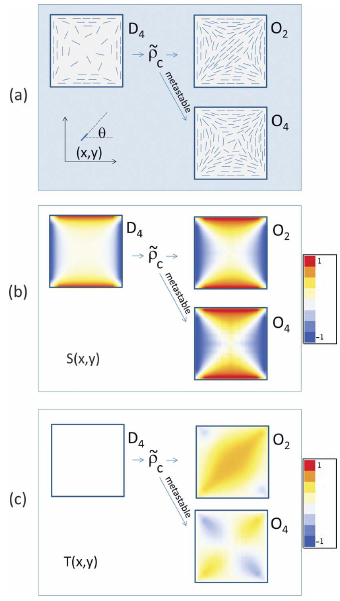
\includegraphics[height=0.86\textheight]{chen2013_ST.png}
	\caption{Stable D and metastable X solutions found in Ref.\ \cite{chen2013rods}. In their work the D state is labeled $O_2$ and the X state is $O_4$, with $D_4$ labeling the isotropic state. $\tilde{\rho}_c$ indicates a transition past the critical transition density. Order parameters $S$ and $T$ are also given. $T$ presents itself as an effective way to distinguish these two topologies.}
	\label{fig:TSmap}
\end{figure}

An intensity map of $T$ and $S$ on the stable diagonal D and metastable X solutions in Figure \ref{fig:TSmap} show how these parameters can be used to characterize different topologies.

Should we wish to determine a bulk nematic order parameter (which we do), we may take the mean values of $S(x,y)$ and $T(x,y)$,
\begin{align}
	\overline{S}(x,y) = \int_{-a/2}^{a/2} \int_{-a/2}^{a/2}\frac{S(x,y)}{a^2} dxdy,
\end{align}
\begin{align}
\overline{T}(x,y) = \int_{-a/2}^{a/2} \int_{-a/2}^{a/2}\frac{T(x,y)}{a^2} dxdy,
\end{align}
for box edge length $a$. In both cases, boundary effects will be annulled since rods order themselves parallel to wall edges \cite{wallordering}. A bulk order parameter 
\begin{align}
	\overline{\Lambda} \equiv \sqrt{\overline{S}^2 + \overline{T}^2}
\end{align}
may then be utilized to gauge if the whole system is in a nematic or isotropic state.

\begin{figure}
	\centering
	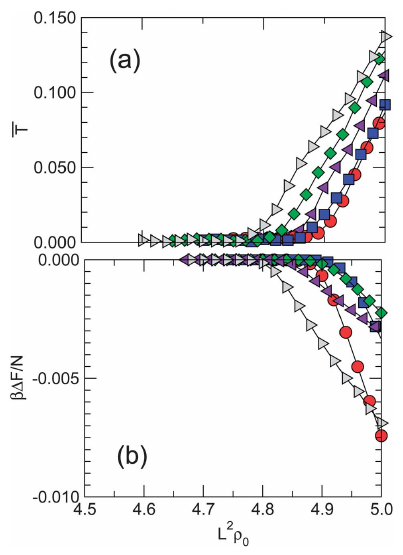
\includegraphics[height=0.55\textheight]{chen2013_Tavg}
	\caption{$\overline{T}$ as function...from \cite{chen2013rods}}
\end{figure}

\begin{figure}
	\centering
	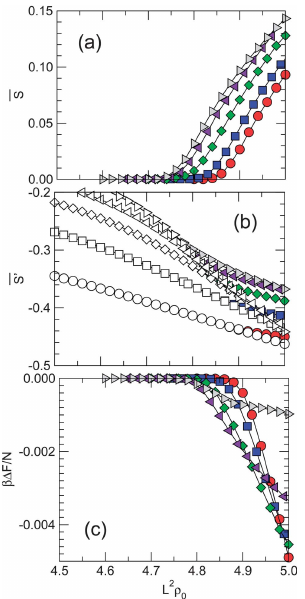
\includegraphics[height=0.8\textheight]{chen2013_Savg}
	\caption{$\overline{S}$ as function...\cite{chen2013rods}}
\end{figure}






